\documentclass{article} 

\usepackage{amsmath}
\usepackage{amssymb}
\usepackage{amsthm}

\newtheorem{lemma}{Lemma}
\newtheorem{theorem}{Theorem}
\newtheorem{corrolary}{Corrolary}

\usepackage[T1]{fontenc}
\usepackage{lmodern}
\usepackage[utf8]{inputenc}

\usepackage{tikz}
\usetikzlibrary{arrows}

\usepackage{caption}
\usepackage{subcaption}

\usepackage{../tex/mathpartir}

\newcommand{\concat}{\ensuremath{+\!\!\!\!+\,}}
\newcommand{\cov}{\vartriangleleft}
\newcommand{\unit}[1]{\ \text{#1}}
\newcommand{\nat}{\mathbb{N}}
\newcommand{\suchthat}{\ |\ }
\newcommand{\List}[1]{\mathsf{list}\ {#1}}
\newcommand{\rat}{\mathbb{Q}}
\newcommand{\R}{\mathbb{R}}
\newcommand{\bool}{\mathbb{B}}
\newcommand{\Prop}{\mathcal{P}}
\newcommand{\Pt}{\mathsf{Pt}}
\newcommand{\irule}[1]{\textsc{#1}}

\title{Programming on continuous spaces}
\author{Ben Sherman}

\date{May 3, 2016}

\begin{document}
\maketitle

\section{Introduction}

Space, time, magnitude, and infinite streams of data are well-modeled by continuous spaces. We may wish to write computer programs which manipulate these concepts, and so desire a programming language which faithfully represents these concepts. Such a language would make it easier to understand the (extensional) behavior of such programs, which is particularly useful in the context of theorem proving.

I am building a Coq framework for reasoning about probability, whose concepts are most naturally expressed in the language of topology. Accordingly, I am also formalizing a theory of topology called \emph{formal topology}; its constructive nature means that formal topology can also be viewed as a programming language embedded in Coq in which data types correspond to topological spaces, and functions correspond to continuous maps.

These notes explain how this programming language for topology works, and how we can use it to solve the following task: \footnote{What does ``arbitrary'' mean? For now I will leave its interpretation open. In general, this article seems to make a habit of being unclear, hand-wavy, or sometimes just plain false, in support of the larger purpose of conveying the general idea of formal topology without getting bogged in the details. Some of these copious footnotes try to clarify the unclear and correct the errors, at the cost of perhaps getting mired in the details.}
\begin{quote}
Given an ``arbitrary'' $f : [0,1] \to \R$, find the maximum value that it attains.
\end{quote}

\section{The real numbers}

The real numbers, $\R$, are one of the most interesting topological spaces, and many computer programs operate on data which are meant to represent real numbers. A common solution is to use floating point numbers rather than $\R$, but programming languages provide few guarantees as to how faithfully programs written using floating point numbers represent the idealized programs that operate on $\R$. Designing floating point computations which do provide such guarantees is a daunting task, and reasoning about the difference between the floating point and the idealized computations is challenging.

Mathematically, the real numbers are defined as sequences of rational approximations, $x : \nat \to \rat$, which are coherent and ever-narrowing; for instance, the $x(n)$ may approximate $x$ to within a distance $1/n$. \footnote{Formally, they satisfy a condition such as: for all $m, n : \nat$, $|x(m) - x(n)| \le 1/m + 1/n$.} It is possible to use this encoding to faithfully represent real numbers as higher-order functions in a programming language. Note that different sequences may represent the same real number. Then a function $f : \R \to \R$ in fact is a transformer of sequences, $f : (\nat \to \rat) \to (\nat \to \rat)$.

It is a remarkable fact that, as long as real numbers $x : \nat \to \rat$ may be black boxes where one can only learn about them by querying for approximations $x(n)$, then any computable function $f$ must be continuous. Given some $x : \R$ and some desired precision $\varepsilon = 1 / n$, $f$ must compute $f(x)(n)$ in finite time. Therefore, it must only look at finitely many entries of the sequence $x$, so if the maximum index it looks at is $m$, it can only determine $x$ to within $\delta = 1 / m$, and therefore for any other $x'$ whose distance from $x$ is less than $\delta$, the $f(x)$ and $f(x')$ must differ by no more than $\varepsilon$.
\footnote{LEJ Brouwer made this observation and postulated the existence of ``free choice sequences,'' lawless sequences whose values are unconstrained other than at the entries where they have already been observed. As a consequence, he derived \emph{Brouwer's continuity principle}, which states that for every property of sequences $P : (\nat \to \nat) \to \bool$ and every sequence $\alpha : \nat \to \nat$, there is some point at which $P$ stopped inspecting $\alpha$. That is, for some $n : \nat$, it only look at the first $n$ entries of the sequences, such that for every $\beta : \nat \to \nat$ which shares the same length-$n$ prefix as $\alpha$, the result $P(\alpha) = P(\beta)$. As a consequence, he found that all functions on $\R \to \R$ are continuous, and refuted the law of the excluded middle, which says that every logical proposition is either true or false. The concept of ``formal topology'' explained in this article gives a way to give computational meaning to Brouwer's concepts of choice sequences.}

Let's return to the task in the introduction. It's quite difficult using the floating point representation: notice that a function $f : [0,1] \to \R$ might not even \emph{have} a maximum if it is not continuous. Despite the general appeal of providing functionality which would find a maximum over black box functions, not even MATLAB offers a tool to do so; the closest MATLAB comes is in its \texttt{fminbnd} function, which uses advanced numerical techniques to find a \emph{local} maximum of a ``continuous'' floating point function.

If we encode $\R$ as sequences $\nat \to \rat$, the task is still difficult, because even though we are sure $f : \R \to \R$ is continuous, we don't know ``how'' continuous it is, and we have no way to inspect its continuity.
\footnote{We know that $f$, when outputting an approximation, only reads a finite approximation of its input. If we could tell how closely $f$ looks at its input, we \emph{could} actually find the maximum of $f$. In many programming languages, it is possible to use effects such as mutable state or exceptions to inspect how continuous $f$ is. However, without such powers, this is impossible to determine.

This is related to the fact that, using the definitions of point-set topology, the Heine-Borel property, which says that every open cover of the unit interval $[0,1]$ has finite subcover, is undecided in constructive mathematics. Adding either the law of the excluded middle or Brouwer's continuity principle proves the Heine-Borel property, but there is a counterexample in the realizability model. A significant motivation of formal topology is to formulate topology such that there is a constructive proof of the Heine-Borel property.
}

\section{An analogy}

The fact that encoding $\R$ as sequences of approximations forces computable functions $f : \R \to \R$ to be continuous suggests a close connection between computer programs and topology, and that a programming language for continuous spaces might be quite expressive.

There are many analogous concepts in computer programs and topology. If you are familiar with one of the two, but not the other, the following dictionary can effectively give a good intuition for the other one.
\footnote{It may be surprising that functions and values have very different interpretations in topology, given that functions are values in higher-order functional programming languages. The difference is that, for any types $X$ and $Y$, we also have a function type $X \to Y$, but for topological spaces $X$ and $Y$, it may be impossible to create a topological space of functions $X \to Y$ which behaves well enough.}

\begin{table}[h]
\begin{tabular}{c @{\hspace{3em}} l @{\hspace{3em}} l}
 & computer programs & topology \\
\hline \hline
$X$ & data type & topological space \\
$f : X \to Y $ & function & continuous map \\
$x : X$ & value & point \\
$P : X \rightharpoonup \bool$ & ``affirmable'' property (semidecidable) & open subset \\
$P : X \rightharpoondown \bool$ & ``refutable'' property (semidecidable) & closed subset \\
$P : X \to \bool$ & decidable property & clopen subset 
\end{tabular}
\end{table}

An ``affirmable'' property is a property that can be verified by a semidecision procedure: if the property holds, then the procedure will halt and return $\mathsf{true}$, whereas if the property does not hold, the program may never terminate. A ``refutable'' property is a property that can be refuted by a semidecision procedure: if the property doesn't hold, the procedure halts and returns $\mathsf{true}$, whereas if the property does hold, the program may never terminate.

We can intuit some of the fundamental facts of topology by simply translating across the dictionary. For instance,
\begin{theorem}
If $f : X \to Y$ is continuous, and $U \subseteq X$ is open, then $f^{-1}(U) \subseteq X$ (the set of points which $f$ maps to $U$) is open.
\end{theorem}
\begin{proof}
Suppose $P : Y \rightharpoonup \bool$ semidecides membership in $U$. Then the composition $P \circ f : X \rightharpoonup \bool$ semidecides whether $f$ maps a point $x : X$ to $U$, that is, it semidecides membership in $f^{-1}(U)$.
\end{proof}

\begin{theorem}
Finite intersections of open sets are open. (Finite unions of closed sets are closed.)
\end{theorem}
\begin{proof}
Given many semideciders $P_1, \ldots, P_n : X \rightharpoonup \bool$, run each of them and check that they all terminate and return $\mathsf{true}$.
\end{proof}

\begin{theorem}
Countable unions of open sets are open. (Countable intersections of closed sets are closed.)
\end{theorem}
\begin{proof}
Given an enumeration of semideciders $P_1, P_2, \ldots : X \rightharpoonup \bool$, run all of them in parallel (via time-slicing), and halt and return $\mathsf{true}$ if any of the subprograms does so.
\end{proof}

With computational intuition, we observe the subset $U = \{ x \suchthat x > 0 \} \subseteq \R$ is open:
Given $x : \R$ presented as a sequence of approximations, we read each successive approximation, and check whether it is still possible that $x \le 0$. If in fact $x > 0$, then we must also have that for some $\varepsilon > 0$, $x - \varepsilon > 0$, and eventually we will refine our approximation far enough to observe this.

Intuitively, an open set is a property which, when true for a point, is also true in a small vicinity of that point as well.

\section{Formal topology}

We still have yet to provide a framework provides a clear formulation of how to represent continuous spaces, or one which yields a simple solution to the task of maximizing some $f : [0,1] \to \R$.

In this section, we will describe such a framework, which is known as \emph{formal topology}.
\footnote{Formal topology is a theory that was invented in the 1980s to try to give a constructive and predicative account of topology.}
The key idea is to view points in a continuous space as interaction structures: one can iteratively refine one's state of knowledge about a point by asking certain questions and receiving answers. So the interaction involved in determining information about a point is explicit, whereas it is implicit when, say, modeling $\R$ as sequences $\nat \to \rat$ in a functional programming language. Rather than starting with points, and building a topology on top, we will directly formalize the interactions for a given topological space in terms of two notions: \emph{basic opens} and \emph{open covers}. By taking open sets as primitives rather than points, we can force continuous functions to ``explain their work'', which will allow us to maximize a function $f : [0,1] \to \R$.

The \emph{basic opens} of a space are formal objects which are ``rich enough'' to describe the space. 
\footnote{The basic opens should represent a \emph{base} of open sets for the space, which means that any open set can be represented as a union of basic opens.}
For defining the real numbers $\R$ in topology, it suffices to take pairs of rational numbers, $\rat \times \rat$, where a formal open $(p, q)$ (we will additionally require $p < q$) is meant to represent the open interval $(p, q)$.
\footnote{The notational collision of open intervals and pairs is unfortunately confusing in this case, as the pair $(p, q) : \rat \times \rat$ is meant to represent the interval $(p, q) : \R \to \Prop$, but recognizing the distinction between the types is important.}
We can think of basic opens as representing different possible states of knowledge about a point.

\begin{figure}[h]
\begin{center}
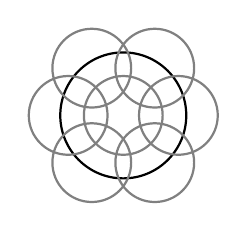
\begin{tikzpicture}
\draw [thick] (2,2) circle (0.8cm);
\draw [thick, gray] (2,2) circle (0.5cm);
\draw [thick, gray] (2.7,2) circle (0.5cm);
\draw [thick, gray] (1.3,2) circle (0.5cm);
\draw [thick, gray] (1.6,2.6) circle (0.5cm);
\draw [thick, gray] (2.4,2.6) circle (0.5cm);
\draw [thick, gray] (1.6,1.4) circle (0.5cm);
\draw [thick, gray] (2.4,1.4) circle (0.5cm);
\end{tikzpicture}
\end{center}
\caption{An open cover}
\end{figure}

In the point-set based topology we previously considered, an open cover $\mathcal{U}$ of an open set $V$ is a collection of open subsets which cover $V$; that is, $V \subseteq \bigcup_{U \in \mathcal{U}} U$. So an open cover is a collection of possible refinements. Intuitively, we can think of an open cover $\mathcal{U}$ of $V$ as a question to ask of a point $x \in V$ that will certainly succeed: since $x$ lies in $V$, if we run the collection of semi-deciders $\mathcal{U}$ in parallel, one will eventually halt, and therefore we will know that for some $U \in \mathcal{U}$, we have $x \in U$. So open covers represent ``safe'' questions to ask of a point to refine our state of knowledge about a point.\footnote{A point may lie in many open sets of an open cover, in which case several responses are possible, and equivalent points may make different choices in their response.}

In formal topology, we \emph{directly axiomatize} the open covers as an inductive type. Given some basic open $a : S$ and a subset $U \subseteq S$, the proposition $a \cov U$ indicates whether $U$ covers $a$, that is, whether $U$ is a ``legitimate question'' to ask of points in $a$.

 For the real numbers, we inductively generate the covering relation by the following rules:
 \footnote{The hypothesis $U \cov V$ in the \irule{transitivity} rule has a subset on the left-hand side; this notation is simply shorthand for $\forall (p, q) \in U, (p, q) \cov V$. Still, the \irule{transitivity} rule looks like it is potentially not well-founded, so one should not interpret these rules directly as the constructors of an inductive type. However, it is possible to inductively generate a cover relation (where the constructors look slightly different) which satisfies all of these rules.}

\begin{figure}[h]
\begin{center}
\begin{subfigure}[t]{0.4\textwidth}
 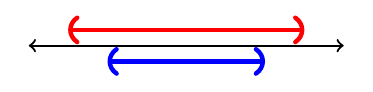
\begin{tikzpicture}
 \draw [<->, thick] (-2, 0) -- (2, 0);
 \draw [(-), ultra thick, blue] (-1, -0.2) -- (1, -0.2);
 \draw [(-), ultra thick, red] (-1.5, 0.2) -- (1.5, 0.2);
 \end{tikzpicture}
\begin{mathpar}
\inferrule* [right=narrow]
  {p' \le p < q \le q' }
  {(p, q) \cov \{(p', q')\}}
\end{mathpar}
\end{subfigure}
~
\begin{subfigure}[t]{0.4\textwidth}
 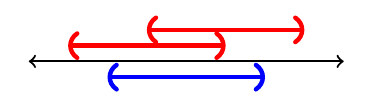
\begin{tikzpicture}
 \draw [<->, thick] (-2, 0) -- (2, 0);
 \draw [(-), ultra thick, blue] (-1, -0.2) -- (1, -0.2);
 \draw [(-), ultra thick, red] (-1.5, 0.2) -- (0.5, 0.2);
  \draw [(-), ultra thick, red] (-0.5, 0.4) -- (1.5, 0.4);
 \end{tikzpicture}
\begin{mathpar}
\inferrule* [right=split]
  {r < p < u < s < q < v}
  {(p, q) \cov \{ (r, s), (u, v) \}}
\end{mathpar}
\end{subfigure}

\vspace{1em}

\begin{subfigure}[t]{0.4\textwidth}
 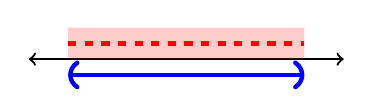
\begin{tikzpicture}
 \draw [<->, thick] (-2, 0) -- (2, 0);
 \draw [(-), ultra thick, blue] (-1.5, -0.2) -- (1.5, -0.2);
 \draw [ultra thick, dashed, red] (-1.5, 0.2) -- (1.5, 0.2);
  \fill[fill=red, opacity=0.2]  (-1.5, 0)--(-1.5,0.4)--(1.5,0.4)--(1.5,0)--(-1.5,0);
 \end{tikzpicture}
\begin{mathpar}
\inferrule* [right=inside]
  { }
  {(p, q) \cov \{ (x, y) \suchthat p < x < y < q \}}
\end{mathpar}
\end{subfigure}

\begin{subfigure}[t]{\textwidth}
\begin{mathpar}
\inferrule* [right=reflexivity]
  { }
  {(p, q) \cov \{(p, q)\}}

\inferrule* [right=transitivity]
  {(p, q) \cov U \\ U \cov V}
  {(p, q) \cov V}
 \end{mathpar}
\end{subfigure}

\end{center}
\end{figure}
 
 The rules \irule{narrow}, \irule{split}, and \irule{inside} describe the structure of the real line, while the rules \irule{reflexivity} and \irule{transitivity} describe the composition structure of valid questions: we can ask a trivially answerable question, and we can chain together questions to form ``plans of investigation'' of a point.

\subsection{Points}
We then define the points of our space as those structures which are able to respond to valid questions. For a space with basic opens $S$, a point $x$ is defined a subset of the basic opens $S$ satisfying certain properties. Intuitively, $x$ is defined as the subset of basic opens which it lies in. We will use the notation $x \models a$ (read ``$x$ lies in a'')\footnote{
The choice of the symbol $\models$ is not accidental. We can read the rules of open covers as a logical sequent calculus, where the basic opens represent propositional variables, and the open cover $a \cov \{u_1, u_2, \ldots\}$ represents
\[
a \vdash u_1, u_2, \ldots
\]
That is, the truth of $a$ implies the truth of either $u_1$, or $u_2$, and so on. Then \irule{reflexivity} corresponds to the identity sequent $a \vdash a$ and \irule{transitivity} represents a sort of infinitary cut rule. Then a point in the space is, by its definition, a model of this logic, assigning consistent truth values to all of the propositional variables.
} for a basic open $a : S$ if $a \in x$. Then a point satisfies the following rules:
\footnote{
A point must satisfy additional properties as well, but this is beyond the scope of this article.
}
\begin{mathpar}
\inferrule* [right=start]
  { }
  {\exists a, x \models a}
  
\inferrule* [right=respond]
  {x \models a \\ a \cov U}
  {\exists b \in U, x \models b}
\end{mathpar}
The \irule{start} rule gives us our starting state of knowledge for a point $x$. Note that there may be a basic open which represents the whole space, and any point may start by saying that it lies in the whole space. The \irule{respond} rule says that if we ask the point $x$ a valid question, we will get a response and update our state of knowledge.

For a point $x$ of $\R$, the \irule{start} rule says that $x$ will initially tell us that it lies in some open interval $(a, b)$. It could be particularly useful to form open covers using \irule{split} and \irule{transitivity}; for instance, we could cover any basic open with open intervals of length $\varepsilon$ in order to approximate a point to within $\varepsilon$.

\subsection{Functions}

In point-set topology, continuous functions $f : \mathcal{X} \longrightarrow \mathcal{Y}$ were those such that for any open set $\mathcal{U} \subseteq \mathcal{Y}$, the set $f^{-1}(\mathcal{U})$ (the set of points which map to $\mathcal{U}$ under $f$) is open.

Since opens are now the primitive objects, we will simply directly define the continuous functions by their inverse images. For formal spaces with basic opens $S$ and $T$, a continuous function $f$ from the space on $S$ to the space on $T$ is a relation $f^{-1}$ where, for a basic open $t : T$, $f^{-1}(t) \subseteq S$ represents the basic opens which map to $t$ under $f$.

The computational meat of continuous functions is that they are question/response transformers, satisfying the following rule, where $a : S$ and $U \subseteq S$:
\footnote{For a subset $U$, we define $f^{-1}(U) = \{ c \suchthat b \in U, c \in f^{-1}(b) \}$.}
\begin{mathpar}
\frac{a \cov_T U}
       {f^{-1}(a) \cov_S f^{-1}(U)}
\end{mathpar}

That is, a continuous function transforms questions about its outputs into questions about its inputs!

\section{Maximizing a function $f : [0,1] \to \R$}

Using formal topology, we are now able to solve the initially posed task: to maximize a black-box function $f : [0,1] \to \R$.

We shall be bold, and try to implement the maximum point $y = \max_{x \in [0, 1]} f(x)$ by implementing its two rules, \irule{start} and \irule{respond}. To simplify the problem, we can assume that we have allowed a basic open $\top_\R$ which represents the whole space, so that our point implements the \irule{start} with this basic open.

Now, suppose that $y$ is issued a question $\top_\R \cov U$, so $y$ must respond with which interval $(p, q) \in U$ it lies in. For concreteness, we might imagine that $U$ is a covering of the real line using infinitely many intervals of the small width $\varepsilon$. Which interval should $y$ pick? Intuitively, it should pick the highest one possible, i.e., the highest interval that $f$ actually reaches. Using the fact that $f$ is a question transformer, we transform this cover into $f^{-1}(\top_R) \cov f^{-1}(U)$, i.e., $[0, 1] \cov f^{-1}(U)$.
\footnote{Note that here we have what appears to be a closed set on the left-hand side of the basic cover. Given that the complement of $[0,1]$ is the open set $\bigcup \{(-\infty, 0), (0, \infty)\}$, the notation $[0,1] \cov f^{-1}(U)$ in fact means
\[
\top_\R \cov \{(-\infty, 0), (0, \infty)\} \cup f^{-1}(U).
\]
}
The Heine-Borel property states that any open cover of the closed interval must have finite subcover. In formal topology, we can actually \emph{compute} this finite subcover by induction on the derivation of the cover. In this specific case, we can compute some finite $V$ such that $f^{-1}(V) \subseteq f^{-1}(U)$ (we can also choose $V$ such that for all $v \in V$, $f^{-1}(v)$ is inhabited).

Now we have a finite set $V$ of open intervals where each open interval $(a, b) \in V$ is reached by $f$. We can simply iterate over the intervals in $V$ and choose the interval with the highest maximum. So the point $y = \max_{x\ \in [0,1]} f(x)$ will say that it lies in that basic open, and is able to successfully implement the \irule{respond} rule. In the specific case where the point $y$ is asked to respond to an open cover of intervals of width $\varepsilon$, the response will approximate $y$ to within $\varepsilon$!

\section{Conclusion}

What have we gained by describing topological spaces using formal topology? At this point, it may not seem that being able to maximize a function $f : [0, 1] \to \R$ justifies the conceptual overhead (while it is a neat trick!). But stepping back from this example, we see that there are benefits to redefining topology in a style amenable to type theory. What results is a framework which is
\begin{itemize}
\item \emph{general} enough to represent all ``reasonable''  topological spaces and continuous functions,
\item \emph{executable}, so that programs described as continuous functions can be run,
\item and \emph{semantically faithful}, in that reasoning about ``programs'' in formal topology is just reasoning about continuous functions and spaces themselves.
\end{itemize}

\end{document}

